\documentclass[beamer]{standalone}


\usepackage{tikz}
\usetikzlibrary{positioning,decorations.pathreplacing,decorations.pathmorphing,arrows,fit}
\usetikzlibrary{calc}




\begin{document}

\resizebox{\textwidth}{!}{

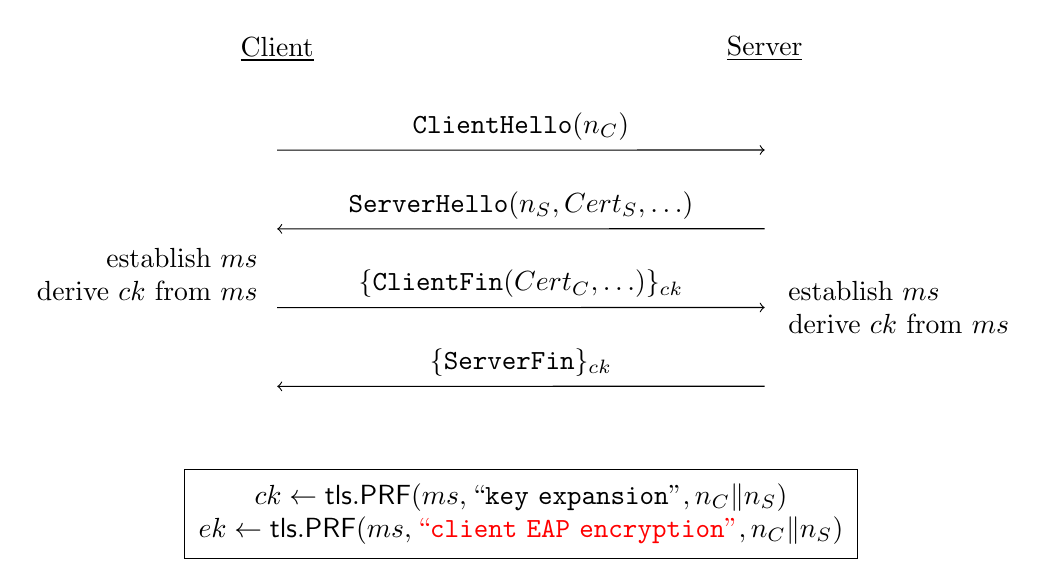
\begin{tikzpicture}[
	    between/.style args={#1 and #2}{
	         at = ($(#1)!0.5!(#2)$)
	    },
    	arrow double line/.style={
    		double distance = 20pt,
       		shorten <= 11, 	
       		shorten >= 16,
       		very thick,
 	    postaction = {
        		draw = white,
 	 	    line width = 20pt,
 	 	    shorten <=-.1pt,
 	 	    shorten >=-.1pt,	
 	    },
 	    postaction = {
    	    	decorate, 
    	    	decoration = {
    	    		markings, 
    	    		mark=at position 0 with {
    	    			\arrow[xshift=26.6pt]{Straight Barb[reversed,length=-1pt 0.7]}
    	    		},
    	    		mark = at position 1 with {
       	    			\arrow[xshift=10.6pt]{Straight Barb[length=-1pt 0.7]}
       	    		}
    	    	}
 	    }
    	},
	]
	

	\node (client) {\underline{Client}};
	\node[right=5cm of client] (server) {\underline{Server}};
	
	\coordinate[below = of client] (c1) {};
	\coordinate[below = 2 of client] (c2) {};
	\coordinate[below = 3 of client] (c3) {};
	\coordinate[below = 4 of client] (c4) {};
	\coordinate[below = of server] (s1) {};
	\coordinate[below = 2 of server] (s2) {};
	\coordinate[below = 3 of server] (s3) {};
	\coordinate[below = 4 of server] (s4) {};
	\coordinate[between = c4 and s4] (midpoint) {};
	
	
	\draw[->] (c1) -- node[above] {$\mathtt{ClientHello}(n_C)$} (s1);
	\draw[<-] (c2) -- node[above] {$\mathtt{ServerHello}(n_S, Cert_S, \dots)$} (s2);
	\draw[->] (c3) -- node[above] {$\lbrace \mathtt{ClientFin}(Cert_C, \dots) \rbrace_{ck}$} (s3);
	\draw[<-] (c4) -- node[above] {$\lbrace \mathtt{ServerFin} \rbrace_{ck}$} (s4);
	

	\node[below left = 5pt of c2,align=right] {establish $ms$\\derive $ck$ from $ms$};
	
	\node[right= 5pt of s3,align=left] {establish $ms$\\derive $ck$ from $ms$};
	

	\node[draw, below=30pt of midpoint,inner sep = 5pt,align=center] {$ck \gets \mathsf{tls.PRF}(ms,``\mathtt{key\ expansion}", n_C \Vert n_S)$\\$ek \gets \mathsf{tls.PRF}(ms,\textcolor{red}{``\mathtt{client\ EAP\ encryption}"}, n_C \Vert n_S)$};


\end{tikzpicture}

}

\end{document}
